\documentclass[10pt,a4paper,twocolumn]{article}
\usepackage[T1]{fontenc}
\usepackage[utf8]{inputenc}
\usepackage{minted}
\usepackage{amsmath}
\usepackage{amsfonts}
\usepackage{amssymb}
\usepackage{fancyhdr}
\usepackage{graphicx, wrapfig, subcaption, setspace, booktabs}
\usepackage[font=small, labelfont=bf]{caption}
\usepackage[list=true]{subcaption}
\usepackage{url, lipsum}
\usepackage{hyperref}
\usepackage{listings}
\usepackage[dvipsnames]{xcolor}
\setlength\headheight{60pt}

\renewcommand{\figurename}{Figura}
\graphicspath{{figures/}}
\renewcommand{\headrulewidth}{2pt}
\definecolor{iselcolor}{rgb}{0.60,0.2 , 0.14} 
\renewcommand{\headrule}{\hbox to\headwidth{%
  \color{iselcolor}\leaders\hrule height \headrulewidth\hfill}}

\usepackage{lscape}

\renewcommand{\lstlistingname}{Algoritmo} % adjusts Listings caption and reference lst
\renewcommand{\lstlistlistingname}{Lista de Algoritmos}
\lstdefinelanguage{Kotlin}{
  comment=[l]{//},
  commentstyle={\color{gray}\ttfamily},
  emph={filter, first, firstOrNull, forEach, lazy, map, mapNotNull, println},
  emphstyle={\color{OrangeRed}},
  identifierstyle=\color{black},
  keywords={!in, !is, abstract, actual, annotation, as, as?, break, by, catch, class, companion, const, constructor, continue, crossinline, data, delegate, do, dynamic, else, enum, expect, external, false, field, file, final, finally, for, fun, get, if, import, in, infix, init, inline, inner, interface, internal, is, lateinit, noinline, null, object, open, operator, out, override, package, param, private, property, protected, public, receiveris, reified, return, return@, sealed, set, setparam, super, suspend, tailrec, this, throw, true, try, typealias, typeof, val, var, vararg, when, where, while},
  keywordstyle={\color{NavyBlue}\bfseries},
  morecomment=[s]{/*}{*/},
  morestring=[b]",
  morestring=[s]{"""*}{*"""},
  ndkeywords={@Deprecated, @JvmField, @JvmName, @JvmOverloads, @JvmStatic, @JvmSynthetic, Array, Byte, Double, Float, Int, Integer, Iterable, Long, Runnable, Short, String, Any, Unit, Nothing},
  ndkeywordstyle={\color{BurntOrange}\bfseries},
  sensitive=true,
  stringstyle={\color{ForestGreen}\ttfamily},
}

\begin{document}
\pagestyle{fancy}
\fancyhead{} % clear all header fields
\fancyhead[LO]{
\includegraphics[width=4cm]{logo_DEETC_cor_completo.png}}
\fancyhead[RO]{
\textbf{Keyboard Reader} (\textit{Roulette Game}) \\ 
\footnotesize
Laboratório de Informática e Computadores 2024 / 2025 verão \\
Autores: David Velez / Nuno Sebastião / Pedro Miguens / Rogério Rebelo / Rui Duarte}
\fancyfoot{} % clear all footer fields
\fancyfoot[RO]{\thepage}


O módulo \textit{Keyboard Reader }é constituído por três blocos principais: \textit{i}) o descodificador de teclado (\textit{Key Decode}); \textit{ii}) o bloco de armazenamento (designado por \textit{Ring Buffer}); e \textit{iii}) o bloco de entrega ao consumidor (designado por \textit{Output Buffer}), de acordo com o diagrama representado na Figura~\ref{fig:keyboardReader}. 
Neste caso o módulo \textit{Control}, implementado em software, é a entidade consumidora.

\begin{figure}[!h]
\begin{center}
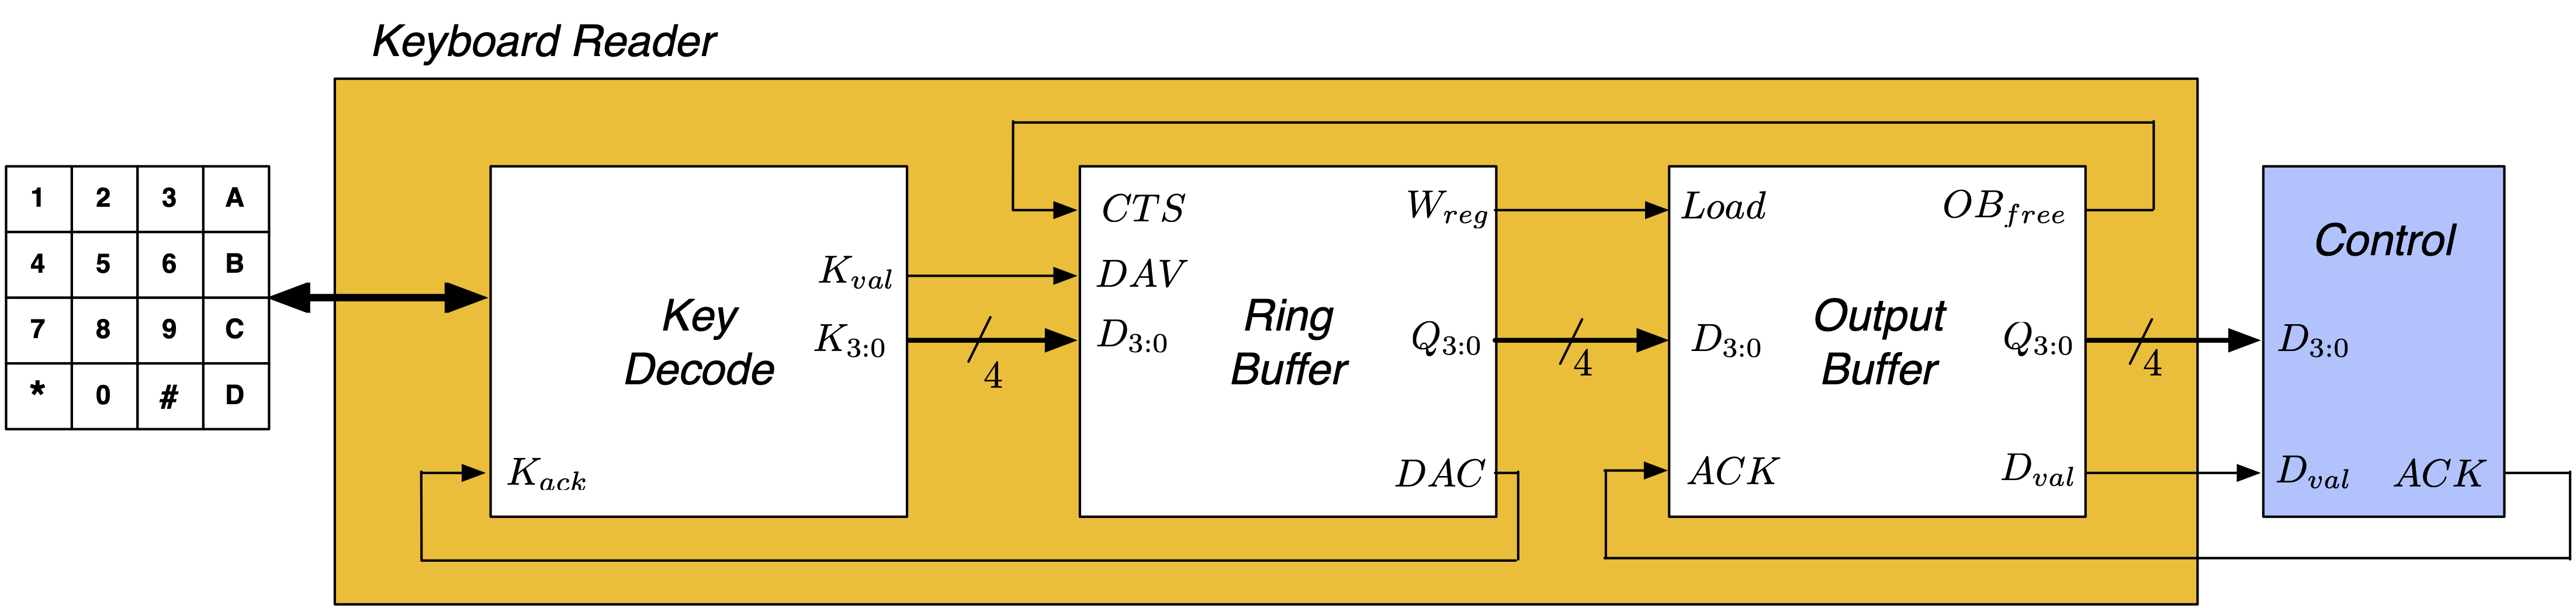
\includegraphics[width=0.48\textwidth]{keyboardReader_diagram.png} 
\caption{Diagrama de blocos do módulo \textit{Keyboard Reader}}
\label{fig:keyboardReader}
\end{center}
\end{figure} 

\section{Key Decode}
O bloco \textit{Key Decode} implementa um descodificador de um teclado matricial 4x3 por hardware, sendo constituído por três sub-blocos: \textit{i}) um teclado matricial de 4x3; \textit{ii}) o bloco Key Scan, responsável pelo varrimento do teclado; e \textit{iii}) o bloco Key Control, que realiza o controlo do varrimento e o controlo de fluxo, conforme o diagrama de blocos representado na Figura~\ref{fig:keyDecode_diagram}. 

O controlo de fluxo de saída do bloco \textit{Key Decode} (para o módulo \textit{Key Buffer}), define que o sinal $K_{val}$ é ativado quando é detetada a pressão de uma tecla, sendo também disponibilizado o código dessa tecla no barramento $K_{0:3}$. 
Apenas é iniciado um novo ciclo de varrimento ao teclado quando o sinal $K_{ack}$ for ativado e a tecla premida for libertada. 
O diagrama temporal do controlo de fluxo está representado na Figura~\ref{fig:keyDecode_protocol}.

\begin{figure}[!h]
\centering
\begin{subfigure}{0.5\textwidth}
	\centering
	\includegraphics[width=0.70\textwidth]{keydecode_diagram.png} 
    \caption{Diagrama de blocos}
    \label{fig:keyDecode_diagram}
\end{subfigure}
\begin{subfigure}{0.5\textwidth}
	\centering
	\includegraphics[width=0.50\textwidth]{keydecode_protocol.png} 
    \caption{Diagrama temporal}
    \label{fig:keyDecode_protocol}
\end{subfigure}
\caption{Bloco \textit{Key Decode}}
\label{fig:keyDecode}
\end{figure}

O bloco \textit{Key Scan} foi implementado de acordo com o diagrama de blocos representado na Figura~\ref{fig:keyScan}. 

\textbf{\textcolor{red}{[Adicionar a justificação da opção tomada.]}}

\begin{figure}[!h]
\begin{center}

\includegraphics[width=0.40\textwidth]{dummyFigure.png} 
\caption{Diagrama de blocos do módulo \textit{Key Scan}}
\label{fig:keyScan}
\end{center}
\end{figure} 

O bloco \textit{Key Control }foi implementado pela máquina de estados representada em \textit{ASM-chart} na Figura~\ref{fig:keyControl_ASM}.

\textbf{\textcolor{red}{[Adicionar a descrição da solução apresentada.]}} 

\begin{figure}[!h]
\begin{center}

\includegraphics[width=0.40\textwidth]{dummyFigure.png} 
\caption{Máquina de estados do \textit{Key Control}}
\label{fig:keyControl_ASM}
\end{center}
\end{figure} 

A descrição hardware do bloco \textit{Key Decode} em\textit{ VHDL} encontra-se no Anexo~\ref{sec:keyDecode_VHDL}.

\section{Key Buffer}
O bloco \textit{Ring Buffer} implementa uma estrutura de dados para armazenamento de teclas com disciplina FIFO (\textit{First In First Out}), com capacidade de armazenar até oito palavras de quatro bits.

A escrita de dados no \textit{Ring Buffer} inicia-se com a ativação do sinal $DAV$ (\textit{Data Available}) pelo sistema produtor, neste caso pelo \textit{Key Decode}, indicando que tem dados para serem armazenados. 
Logo que tenha disponibilidade para armazenar informação, o \textit{Ring Buffer }escreve os dados $D_{0:3}$ em memória. 
Concluída a escrita em memória ativa o sinal $DAC$ (\textit{Data Accepted}) para informar o sistema produtor que os dados foram aceites. O sistema produtor mantém o sinal $DAV$ ativo até que $DAC$ seja ativado. 
O \textit{Ring Buffer} só desativa $DAC$ depois de $DAV$ ter sido desativado.

A implementação do \textit{Ring Buffer} é baseada numa memória RAM (\textit{Random Access Memory}). 
O endereço de escrita/leitura, selecionado por put(get), definido pelo bloco \textit{Memory Address Control }(MAC) composto por dois registos, que contêm o endereço de escrita e leitura, designados por putIndex e getIndex respetivamente. 
O MAC suporta assim ações de incPut e incGet, gerando informação se a estrutura de dados está cheia (\textit{Full}) ou se está vazia (\textit{Empty}). 
O bloco \textit{Ring Buffer }procede à entrega de dados à entidade consumidora, sempre que esta indique que está disponível para receber, através do sinal \textit{Clear} To Send (CTS). 
Na Figura 6 é apresentado o diagrama de blocos para a estrutura do bloco \textit{Ring Buffer}.

\section{...}

\section{Conclusões}

\onecolumn
\clearpage
\appendix
\section{VHDL}
\subsection{KeyBoard Reader}
\label{sec:keyboardReader_VHDL}

\subsection{KeyBoard Reader}
\label{sec:keyboardReader_VHDL}
% Inserção de ficheiro de descrição hardware
\begin{minipage}{\linewidth}
\footnotesize
\inputminted{vhdl}{vhdl/ficheiro1.vhd}
\label{vhdl:fichiero1}
\end{minipage}

\subsection{Key Decode}
\label{sec:keyDecode_VHDL}
% Inserção de ficheiro de descrição hardware
\begin{minipage}{\linewidth}
\footnotesize
\inputminted{vhdl}{vhdl/ficheiro2.vhd}
\label{vhdl:fichiero2}
\end{minipage}

\subsection{Key Scan}
\label{sec:keyscan_VHDL}

\subsection{...}

\clearpage
\section{\textit{Kotlin}}
\subsection{HAL}
\lstinputlisting[language=Kotlin, basicstyle=\scriptsize, caption={HAL - Hardware Abstract Layer}, label={lst:HAL}]{kotlin/HAL.kt}
\subsection{KBD}
\lstinputlisting[language=Kotlin, basicstyle=\scriptsize, caption={KBD}, label={lst:KBD}]{kotlin/KBD.kt}


\end{document}